% Exact gambler's-ruin probability h_k, N=5.
% Fair: h_k=k/5. Biased p=2/3: h_k=(1-2^(-k))/(1-2^(-5)).
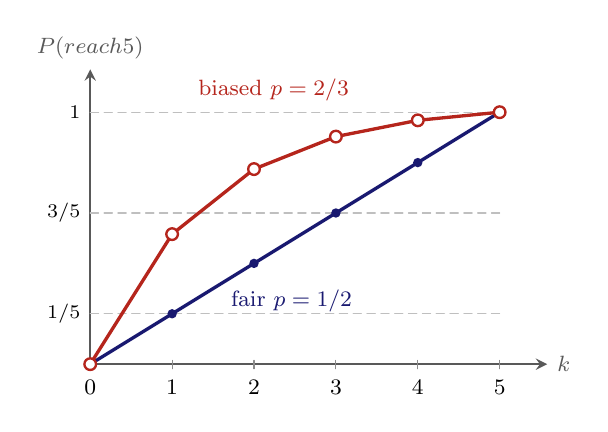
\begin{tikzpicture}[x=1.04cm,y=3.2cm,line cap=round,>=stealth]
  \draw[->,black!65,thick] (0,0)--(5.58,0) node[right,font=\footnotesize] {$k$};
  \draw[->,black!65,thick] (0,0)--(0,1.17) node[above,font=\footnotesize] {$P(\text{reach }5)$};
  \foreach \k in {0,1,2,3,4,5}{
    \draw[black!45] (\k,0.015)--(\k,-0.018);
    \node[below,font=\footnotesize] at (\k,-0.025) {$\k$};
  }
  \foreach \y/\lab in {0.2/{1/5},0.6/{3/5},1/{1}}{
    \draw[black!25,densely dashed] (0,\y)--(5,\y);
    \node[left,font=\scriptsize] at (0,\y) {$\lab$};
  }
  \draw[MidnightBlue,very thick] plot coordinates {(0,0) (1,0.2) (2,0.4) (3,0.6) (4,0.8) (5,1)};
  \draw[BrickRed,very thick] plot coordinates {(0,0) (1,0.5161290323) (2,0.7741935484) (3,0.9032258065) (4,0.9677419355) (5,1)};
  \foreach \k/\y in {0/0,1/0.2,2/0.4,3/0.6,4/0.8,5/1}{
    \fill[MidnightBlue] (\k,\y) circle (1.7pt);
  }
  \foreach \k/\y in {0/0,1/0.5161290323,2/0.7741935484,3/0.9032258065,4/0.9677419355,5/1}{
    \draw[BrickRed,fill=white,line width=0.85pt] (\k,\y) circle (2.1pt);
  }
  \node[font=\footnotesize,anchor=west,text=MidnightBlue] at (1.6,0.25) {fair $p=1/2$};
  \node[font=\footnotesize,anchor=west,text=BrickRed] at (1.2,1.09) {biased $p=2/3$};
\end{tikzpicture}
